\documentclass[11pt]{article}

\usepackage{booktabs}
\usepackage{homeworkpkg}
\usepackage{enumitem}
\usepackage{xcolor,listings}
\usepackage{caption}
\usepackage{multirow}
\usepackage{multicol}

\graphicspath{ {../results/} }

%% Local Macros and packages: add any of your own definitions here.

\begin{document}

% Homework number, your name and NetID, and optionally, the names/NetIDs of anyone you collaborated with. If you did not collaborate with anybody, leave the last parameter empty.
\homework
    {4}
    {Nestor Alejandro Bermudez Sarmiento (nab6)}
    {}

\section*{Introduction}

Assignment 4 covers the topics of Perceptrons and Q-learning by implementing a digit classifier (from the same data as for Assignment 3) and a game of Pong, respectively. The first part is about the digit classification problem; $k$-nearest neighbor and perceptron classifiers will be implemented. In the second part I'll discuss the implementation using reinforcement learning to train the agent to play Pong. \\

As in the previous assignments, I'll be using Python 3.6. 

\section*{Part 1}

Since we will be using the same data set we used in Assignment 3 I'll reuse some of the classes I created previously; namely:
\begin{enumerate}
\item \textbf{Parser}: class to read the data files and create an internal representation. 

\item \textbf{FeatureExtractors}: takes the original data and create features from it, be it: binarize it, group pixels or use a ternary feature. 

\item \textbf{Utilities}: helper methods to print out matrices, create the color maps and scatter plots. 
\end{enumerate}

\subsection*{Part 1.1}

For this part I have implemented a new classifier class called \textbf{PerceptronClassifier}. The interface is pretty much the same as for the previously developed classifiers: it has \textit{train} and \textbf{evaluate} methods that create the training curve and confusion matrix respectively. \\
The classifier accepts the following parameters: 
\begin{enumerate}
\item \textbf{epochs}: number of iterations until convergence of the weights.

\item \textbf{shuffle}: a boolean flag that indicates whether the training examples will be used in a fixed order or randomized.

\item \textbf{use\_bias}: a boolean flag that indicates whether we should augment our features to generate a $\beta_0$ weight, a.k.a. bias. If the bias is used then the features are "augmented" with an additional dimension with value 1. 

\item \textbf{zero\_weights}: a boolean flag that indicates whether the weights should be initialized using all zeros or a random value between 0 and 1.

\item \textbf{learning\_rate\_decay}: a function that dictates how big should the step for the weight update should be. Two different functions were explored: time inverse and exponential decay. The idea for using these was inspired by the available decay functions in Tensorflow\footnote{\url{https://www.tensorflow.org/versions/r0.12/api_docs/python/train/decaying_the_learning_rate}}. 

\item \textbf{learning\_rate}: a constant that may be used by the decay function along with the epoch.
\end{enumerate}

As per the implementation itself, I simply repeat the process for every epoch, on each iteration every example in the training data set is classified using the current weights and if it is misclassified then the corresponding weights are updated based on the decay function, learning rate constant and the example in question.\\

Multiple configurations of the parameters were tried and the best was chosen. The following table contains a summary of the different parameters and the corresponding results.

\begin{center}
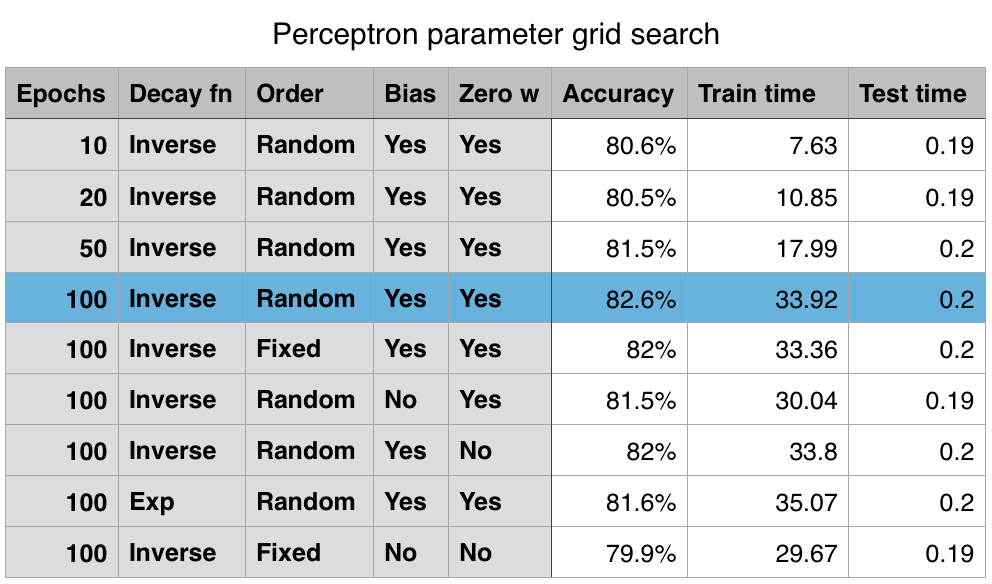
\includegraphics[scale=0.7]{part1.1/params.png}
\captionof{table}{Different parameters for perceptron classifier}
\end{center}

Now, lets look at the corresponding confusion matrix for the best accuracy obtained: 100 epochs, time inverse decay function, random process of examples, with bias and zero initialized weights.

\begin{center}
  \begin{tabular}{cc|r|r|r|r|r|r|r|r|r|r|l}
  \cline{3-12}
  & & \multicolumn{10}{ c| }{Predicted class} \\ \cline{3-12}
  & & 0 & 1 & 2 & 3 & 4 & 5 & 6 & 7 & 8 & 9  \\ \cline{1-12}
  \multicolumn{1}{ |c  }{\multirow{10}{*}{Class} } &
  \multicolumn{1}{ |r| }{0} & 94.44 & 0 & 1.11 & 0 & 0 & 0 & 1.11 & 0 & 2.22 & 1.11    \\ \cline{2-12}
  \multicolumn{1}{ |c  }{}                        &
  \multicolumn{1}{ |c| }{1} & 0 & 97.22 & 0.93 & 0 &  0.93 & 0 & 0.93 & 0 & 0 & 0    \\ \cline{2-12}
  \multicolumn{1}{ |c  }{}                        &
  \multicolumn{1}{ |c| }{2} & 0 & 1.94 & 83.50 & 3.88 &  1.94 & 0 & 3.88 & 2.91 & 1.94 & 0    \\ \cline{2-12}
  \multicolumn{1}{ |c  }{}                        &
  \multicolumn{1}{ |c| }{3} & 0 & 0 & 2 & 80 &  0 & 9 & 2 & 4 & 3 & 0    \\ \cline{2-12}
  \multicolumn{1}{ |c  }{}                        &
  \multicolumn{1}{ |c| }{4} & 0 & 0 & 3.74 & 0.93 &  82.24 & 0 & 2.8 & 2.8 & 0 & 7.48    \\ \cline{2-12}
  \multicolumn{1}{ |c  }{}                        &
  \multicolumn{1}{ |c| }{5} & 2.17 & 0 & 1.09 & 6.52 &  0 & 78.26 & 0 & 3.26 & 6.52 & 2.17    \\ \cline{2-12}
  \multicolumn{1}{ |c  }{}                        &
  \multicolumn{1}{ |c| }{6} & 1.1 & 1.1 & 2.2 & 0 &  2.2 & 2.2 & 86.81 & 2.2 & 2.2 & 0    \\ \cline{2-12}
  \multicolumn{1}{ |c  }{}                        &
  \multicolumn{1}{ |c| }{7} & 0.94 & 2.83 & 3.77 & 1.89 &  2.83 & 0 & 0 & 77.36 & 0.94 & 9.43    \\ \cline{2-12}
  \multicolumn{1}{ |c  }{}                        &
  \multicolumn{1}{ |c| }{8} & 0 & 1.94 & 6.8 & 7.77 & 1.94 &  4.85 & 2.91 & 0.97 & 68.93 & 3.88    \\ \cline{2-12}
  \multicolumn{1}{ |c  }{}                        &
  \multicolumn{1}{ |c| }{9} & 0 & 0 & 1 & 6 &  8 & 1 & 0 & 5 & 1 & 78    \\ \cline{1-12}
  \end{tabular}
  \captionof{table}{Confusion matrix. Values are percentages.}
\end{center}

Overall accuracy: \textbf{82.6\%}. We can see that the performance of this classifier is better than the Naive Bayes classifier using single pixels as features that I created for Assignment 3. With Naive Bayes the best accuracy achieved was \textbf{77.6\%}.\\
By looking at the confusion matrices we can see that the improvement comes from a better accuracy when classifying digits 0 to 7. The accuracy for digits 8 and 9 decreased when using the perceptron classifier.\\

While training the classifier, for every epoch, the classifier was evaluated using the same training data and the accuracy was captured. The following chart captures the progress in the accuracy of the model.

\begin{center}
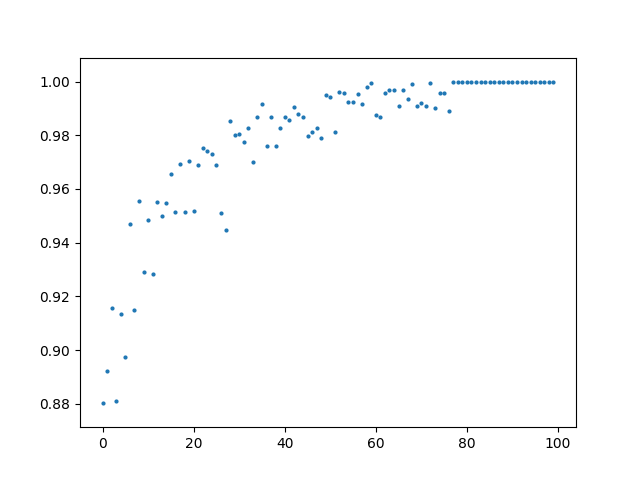
\includegraphics[scale=0.75]{part1.1/trainingcurve/setup4.png}
\captionof{figure}{Accuracy as $k$ increases}
\end{center}

Note: the training curve and confusion matrix was capture for every configuration of parameters and they can be found under the results folder accompanying this report. They are not included in the report because the instructions indicated it was not necessary and for the sake of brevity.

\subsection*{Part 1.2}

In this section we cover the implementation of a $k$-nearest neighbor classifier and compare the results with the previous classifiers.\\

For $k$-nearest neighbor I tuned two parameters: first the value of $k$ and, second, the distance measure used.\\

The values of $k$ were: 1, 2, 3, 5, 7, 13, 23, 43 and 91. And I tried three different distance measurements for each of those $k$. The distance functions are: Euclidean distance, Cosine similarity and Jaccard coefficient. The following charts show how the accuracy changes as a function of $k$ for the different distances.

\begin{center}
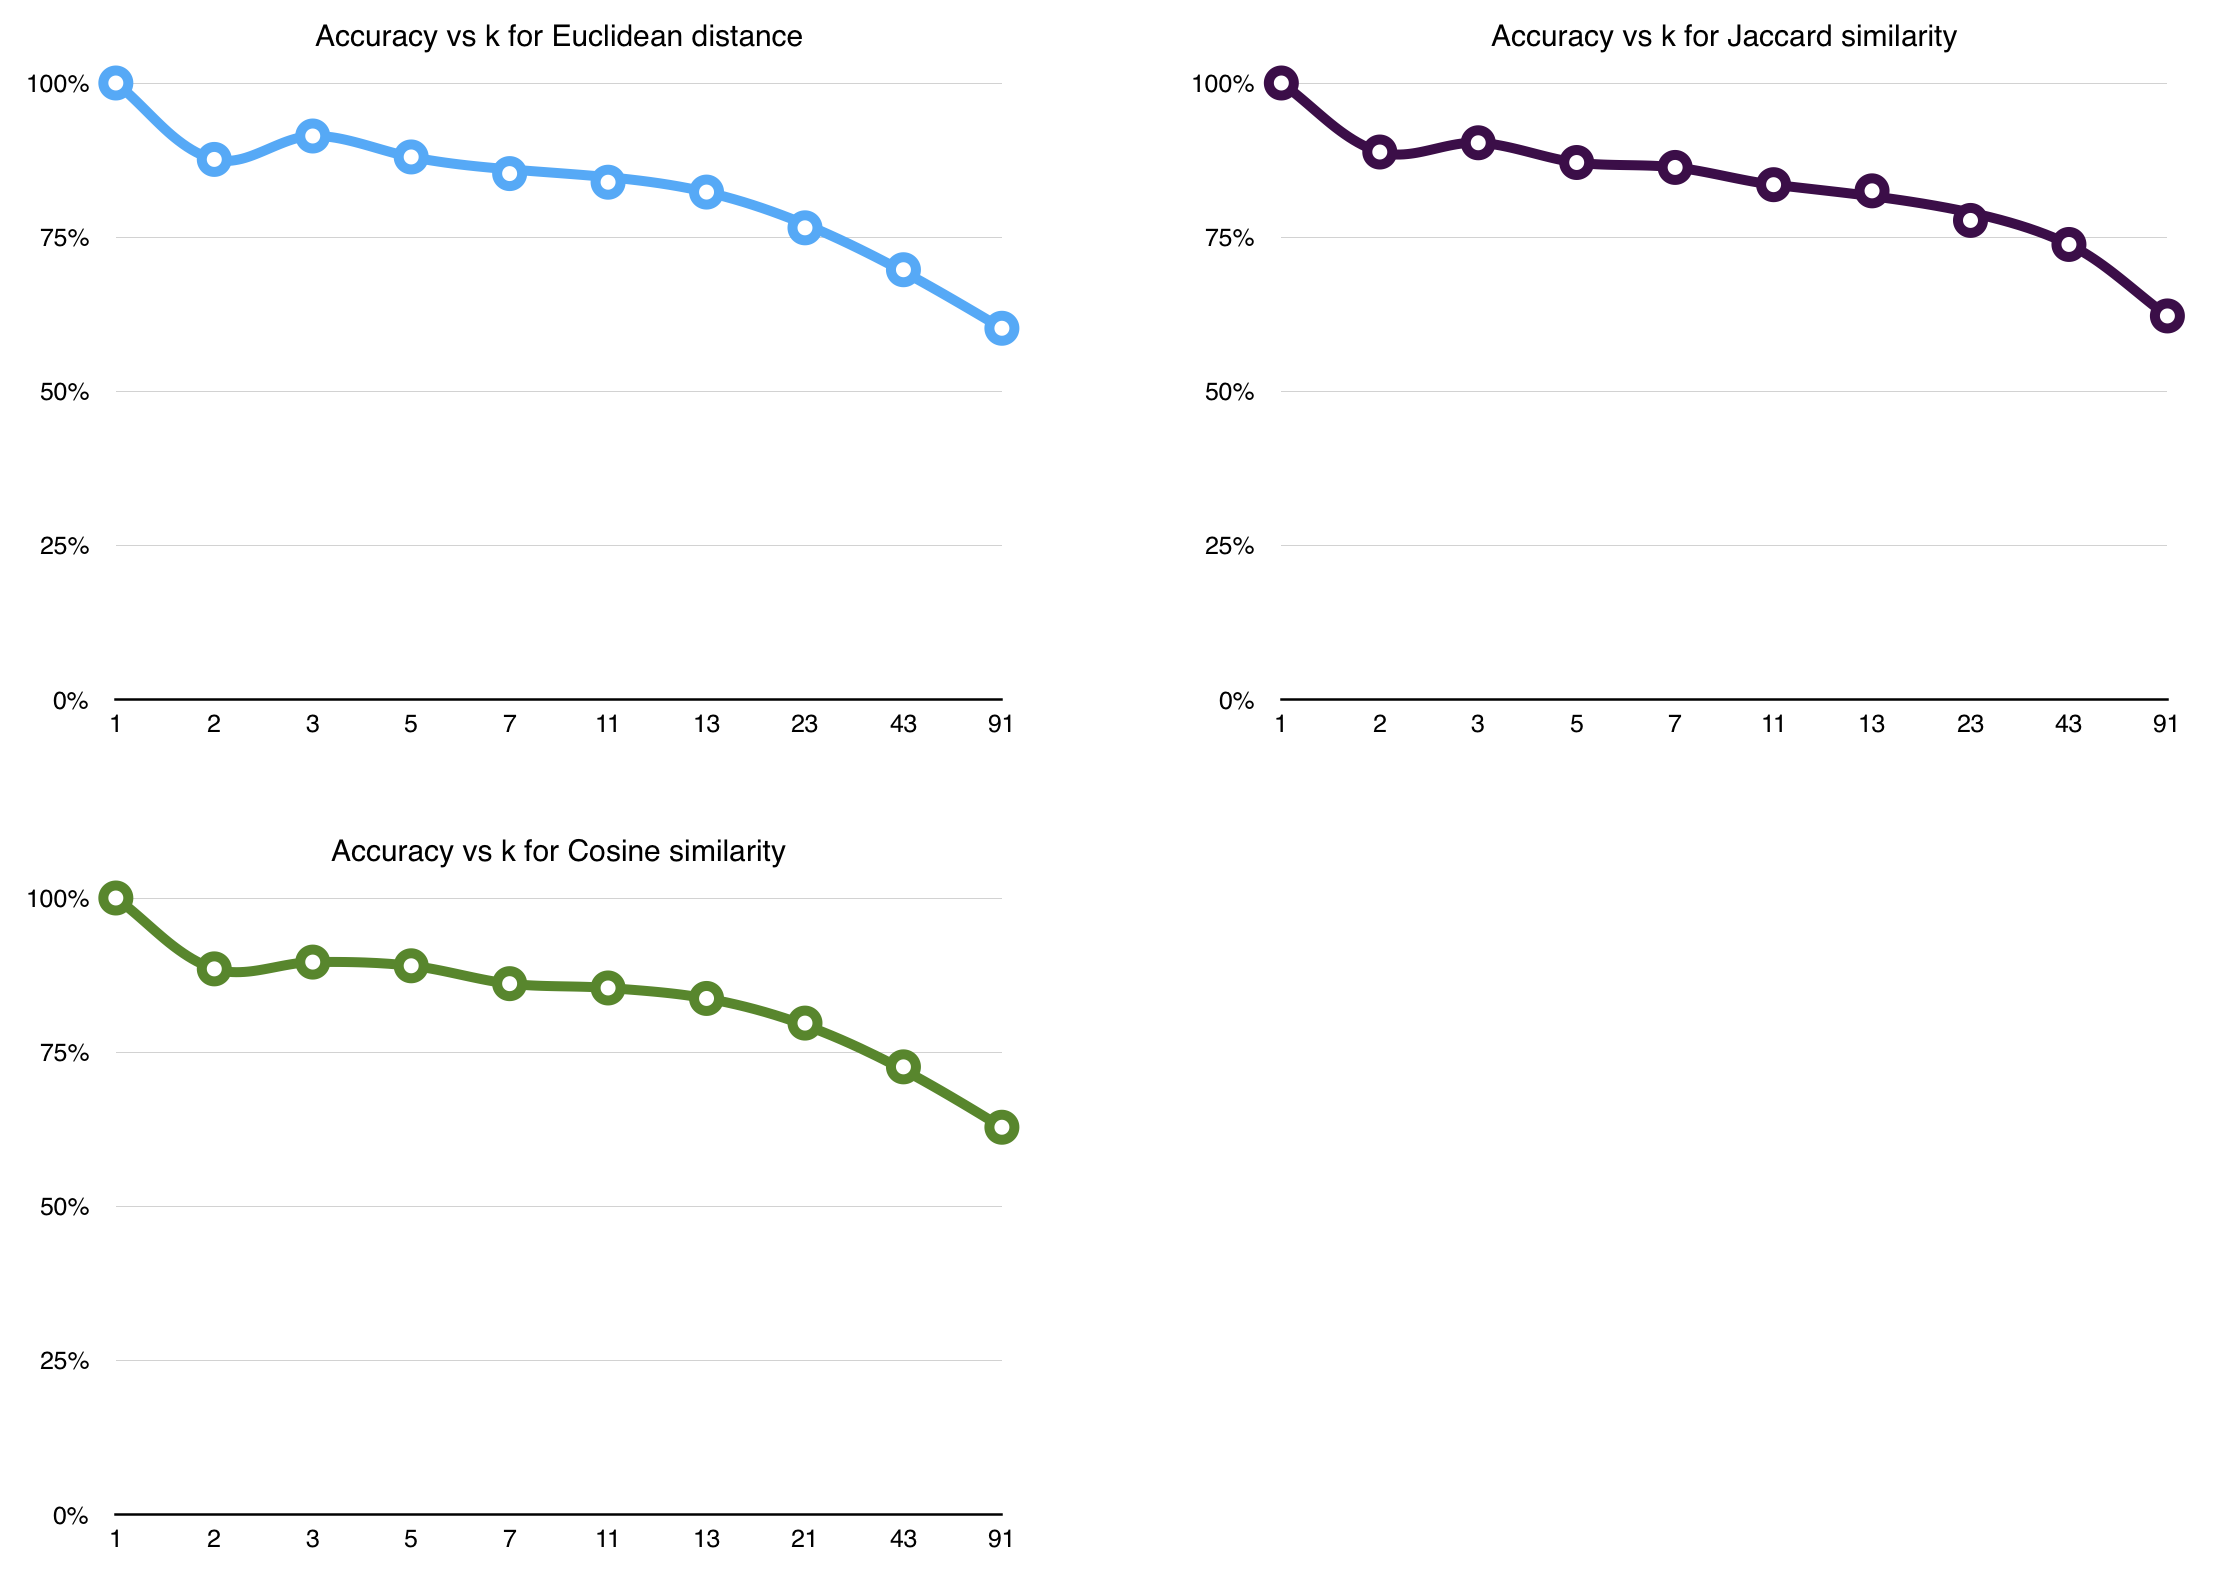
\includegraphics[scale=0.4]{part1.2/acc-vs-k.png}
\captionof{figure}{Accuracy vs $k$}
\end{center}

Notice how the three plots have the same overall shape and they all reach a maximum when using $k=1$. To my surprise, it achieved a \textbf{100\%} accuracy!\\

Now lets look at the time it takes to evaluate the classifier using the testing data set.

\begin{center}
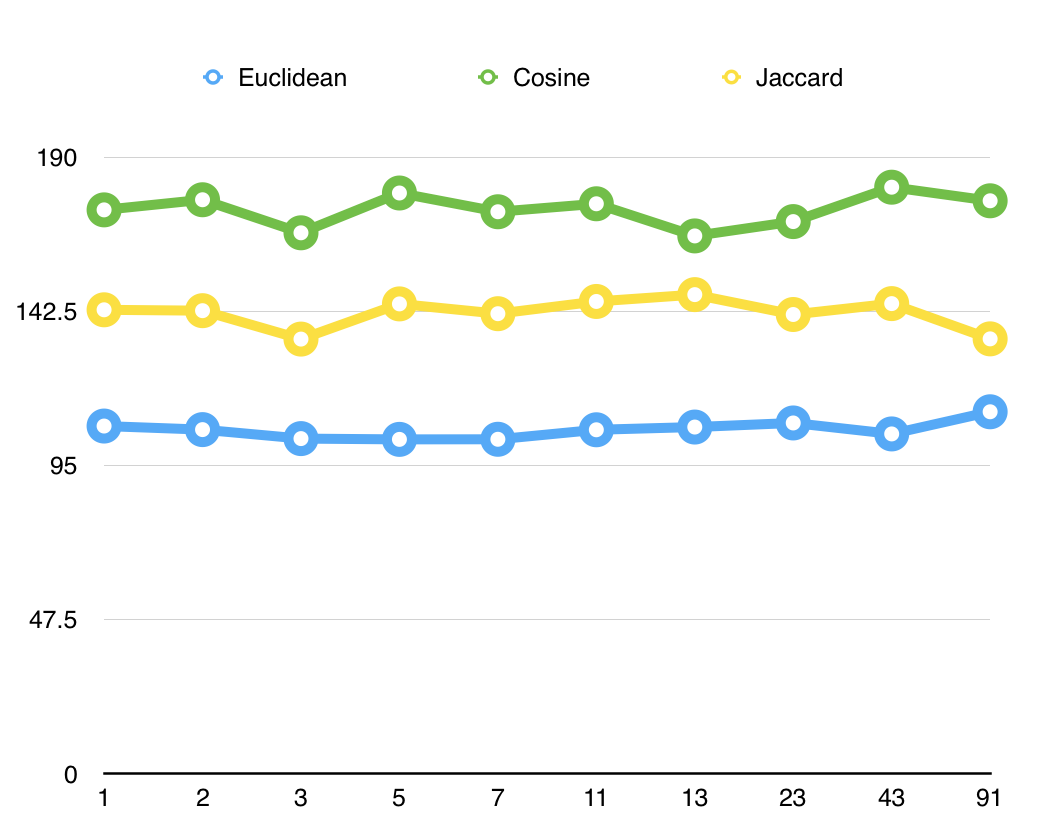
\includegraphics[scale=0.65]{part1.2/test-time.png}
\captionof{figure}{Testing time as a function of $k$}
\end{center}

Out of the three distance measures Euclidean distance is the most efficient one when it comes to test time. Since all three of them achieve 100\% I'll report the confusion matrix when using Euclidean distance. As expected, the confusion matrix would have 100 on its diagonal and 0 everywhere else.

\begin{center}
  \begin{tabular}{cc|r|r|r|r|r|r|r|r|r|r|l}
  \cline{3-12}
  & & \multicolumn{10}{ c| }{Predicted class} \\ \cline{3-12}
  & & 0 & 1 & 2 & 3 & 4 & 5 & 6 & 7 & 8 & 9  \\ \cline{1-12}
  \multicolumn{1}{ |c  }{\multirow{10}{*}{Class} } &
  \multicolumn{1}{ |r| }{0} & 100 & 0 & 0 & 0 & 0 & 0 & 0 & 0 & 0 & 0    \\ \cline{2-12}
  \multicolumn{1}{ |c  }{}                        &
  \multicolumn{1}{ |c| }{1} & 0 & 100 & 0 & 0 & 0 & 0 & 0 & 0 & 0 & 0     \\ \cline{2-12}
  \multicolumn{1}{ |c  }{}                        &
  \multicolumn{1}{ |c| }{2} & 0 & 0 & 100 & 0 & 0 & 0 & 0 & 0 & 0 & 0     \\ \cline{2-12}
  \multicolumn{1}{ |c  }{}                        &
  \multicolumn{1}{ |c| }{3} & 0 & 0 & 0 & 100 & 0 & 0 & 0 & 0 & 0 & 0    \\ \cline{2-12}
  \multicolumn{1}{ |c  }{}                        &
  \multicolumn{1}{ |c| }{4} & 0 & 0 & 0 & 0 & 100 & 0 & 0 & 0 & 0 & 0    \\ \cline{2-12}
  \multicolumn{1}{ |c  }{}                        &
  \multicolumn{1}{ |c| }{5} & 0 & 0 & 0 & 0 & 0 & 100 & 0 & 0 & 0 & 0    \\ \cline{2-12}
  \multicolumn{1}{ |c  }{}                        &
  \multicolumn{1}{ |c| }{6} & 0 & 0 & 0 & 0 & 0 & 0 & 100 & 0 & 0 & 0    \\ \cline{2-12}
  \multicolumn{1}{ |c  }{}                        &
  \multicolumn{1}{ |c| }{7} & 0 & 0 & 0 & 0 & 0 & 0 & 0 & 100 & 0 & 0    \\ \cline{2-12}
  \multicolumn{1}{ |c  }{}                        &
  \multicolumn{1}{ |c| }{8} & 0 & 0 & 0 & 0 & 0 & 0 & 0 & 0 & 100 & 0    \\ \cline{2-12}
  \multicolumn{1}{ |c  }{}                        &
  \multicolumn{1}{ |c| }{9} & 0 & 0 & 0 & 0 & 0 & 0 & 0 & 0 & 0 & 100    \\ \cline{1-12}
  \end{tabular}
  \captionof{table}{Confusion matrix. Values are percentages.}
\end{center}

One important observation is that the testing time is relatively stable given the distance measurement; meaning it doesn't change much as the number $k$ increases. This makes sense because, in order to find the best $k$, you still have to calculate the distance against \textit{all} the training examples. The different in time depends exclusively on the distance function. \\

Finally, it is obvious that $k$-nearest neighbor outperforms both my Naive Bayes and Perceptron classifiers by a wide margin and, when using the same features, Naive Bayes is the one with the lowest accuracy.

\subsection*{Extra credits}

\textbf{Extra Credit 1 - Advanced features}: as done in Assignment 3, I'll now use features that encode a group of pixels of various sizes. The same sizes were used: 2x2, 2x3, 3x2 and 3x3. \\

\begin{center}
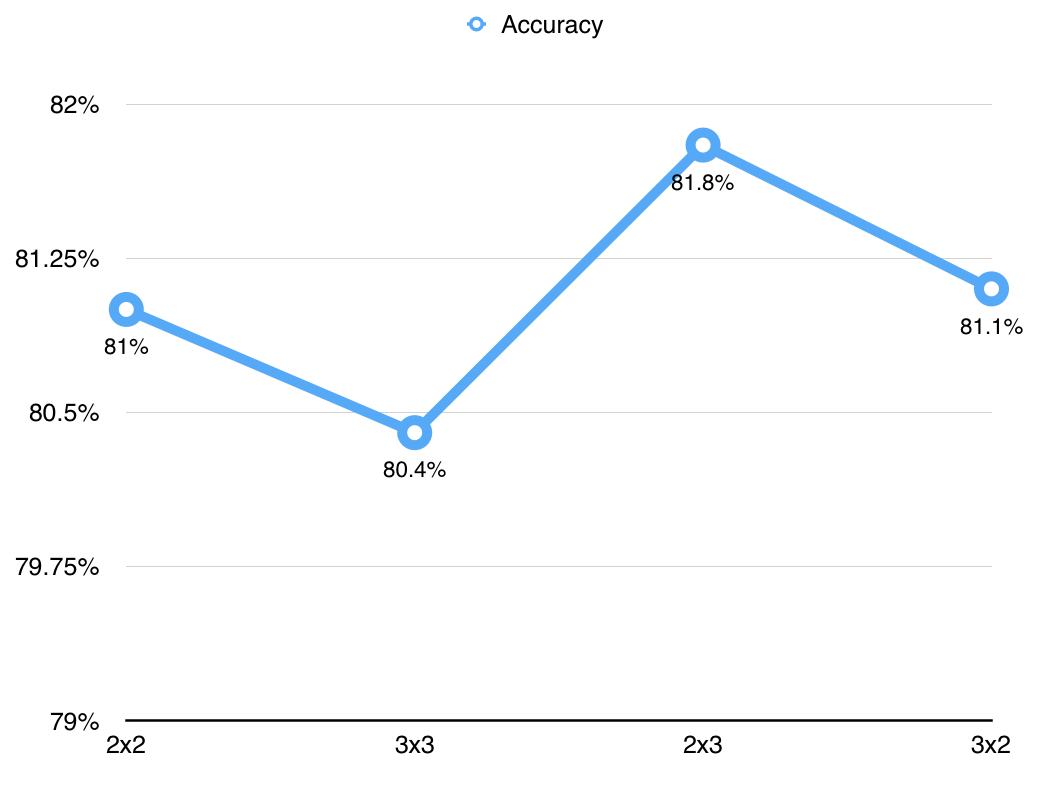
\includegraphics[scale=0.65]{part1.ec1/groups.png}
\captionof{figure}{Accuracy for groups of pixels as features.}
\end{center}

The highest accuracy when using these groups was \textbf{81.6\%} which is still better than the accuracy obtained by Naive Bayes but does not improve the accuracy obtained by using single pixels. Training curves and confusion matrices can be found in the results folder.\\

\textbf{Extra Credit 2 - Weights visualization}: lets look at the color maps of the weights for each of the digits.\\

\begin{center}
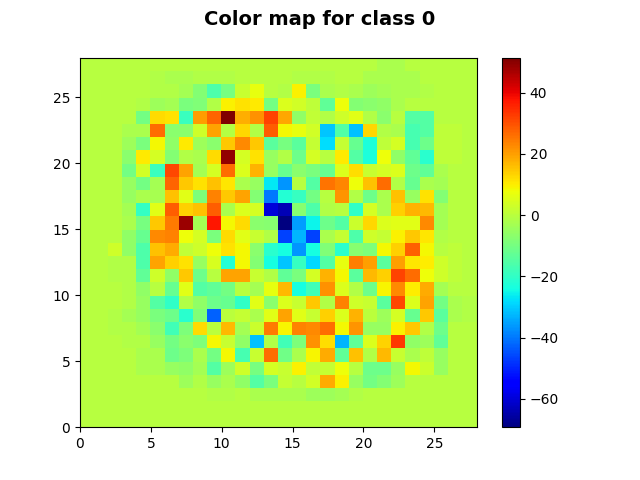
\includegraphics[scale=0.80]{part1.ec2/digit0.png}
\captionof{figure}{Color map for digit 0.}
\end{center}

\begin{center}
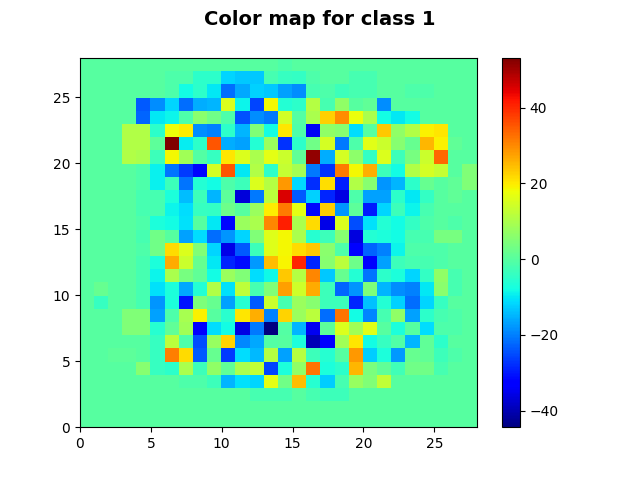
\includegraphics[scale=0.80]{part1.ec2/digit1.png}
\captionof{figure}{Color map for digit 1.}
\end{center}

\begin{center}
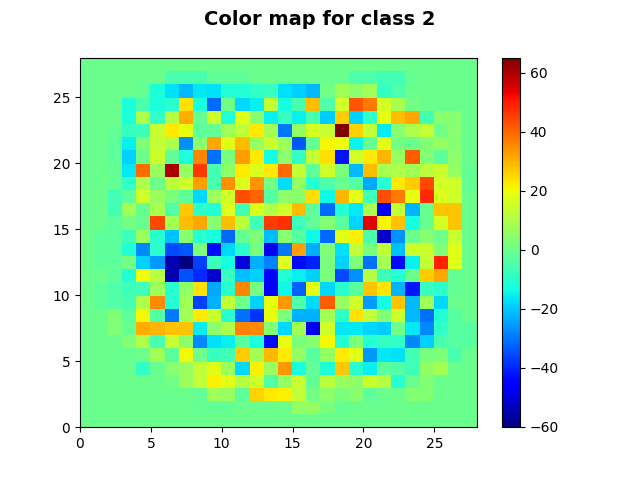
\includegraphics[scale=0.80]{part1.ec2/digit2.png}
\captionof{figure}{Color map for digit 2.}
\end{center}

\begin{center}
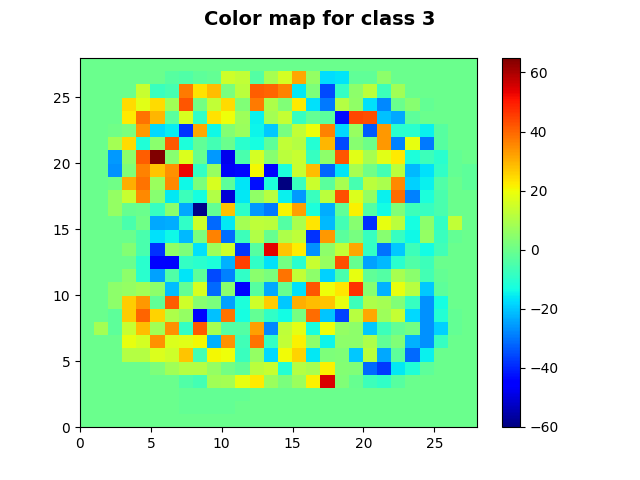
\includegraphics[scale=0.80]{part1.ec2/digit3.png}
\captionof{figure}{Color map for digit 3.}
\end{center}

\begin{center}
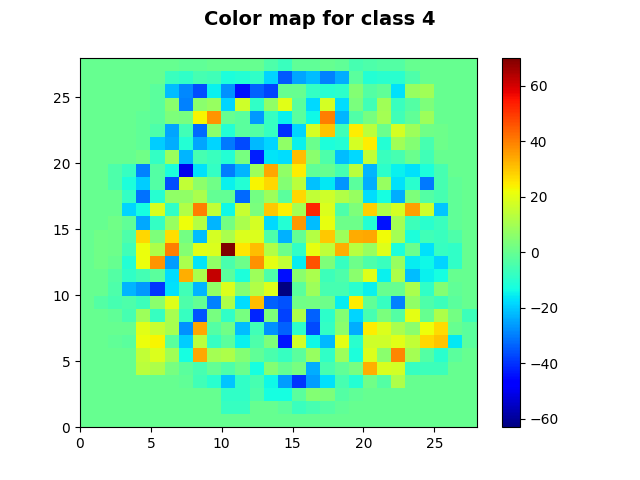
\includegraphics[scale=0.80]{part1.ec2/digit4.png}
\captionof{figure}{Color map for digit 4.}
\end{center}

\begin{center}
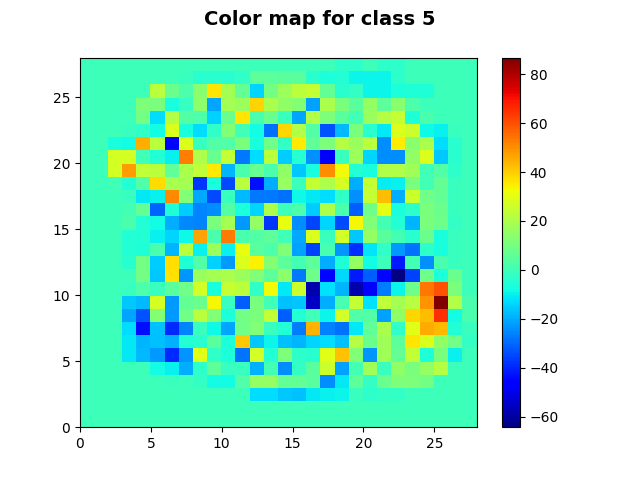
\includegraphics[scale=0.80]{part1.ec2/digit5.png}
\captionof{figure}{Color map for digit 5.}
\end{center}

\begin{center}
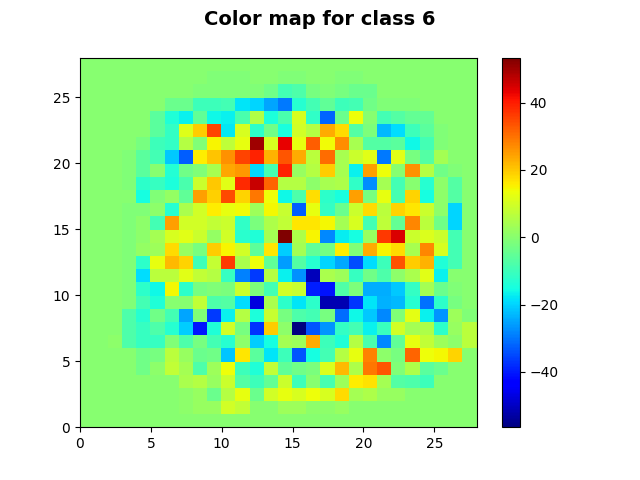
\includegraphics[scale=0.80]{part1.ec2/digit6.png}
\captionof{figure}{Color map for digit 6.}
\end{center}

\begin{center}
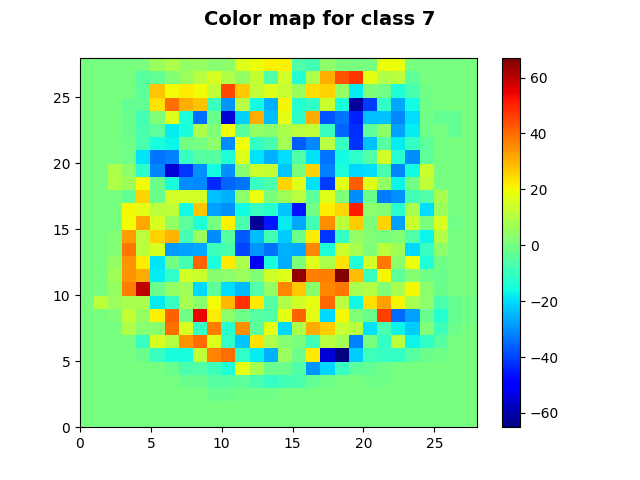
\includegraphics[scale=0.80]{part1.ec2/digit7.png}
\captionof{figure}{Color map for digit 7.}
\end{center}

\begin{center}
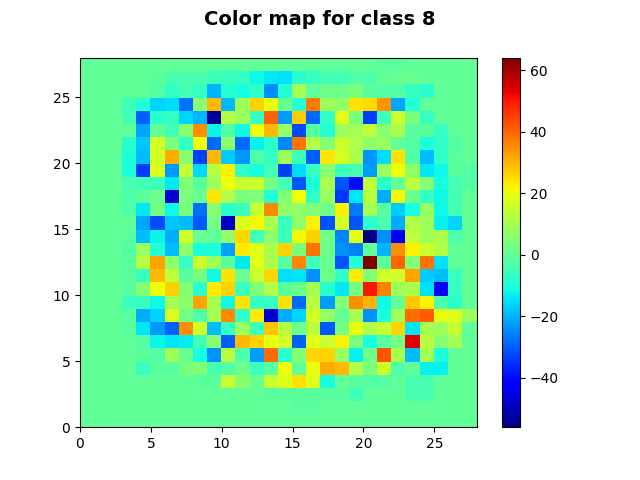
\includegraphics[scale=0.80]{part1.ec2/digit8.png}
\captionof{figure}{Color map for digit 8.}
\end{center}

\begin{center}
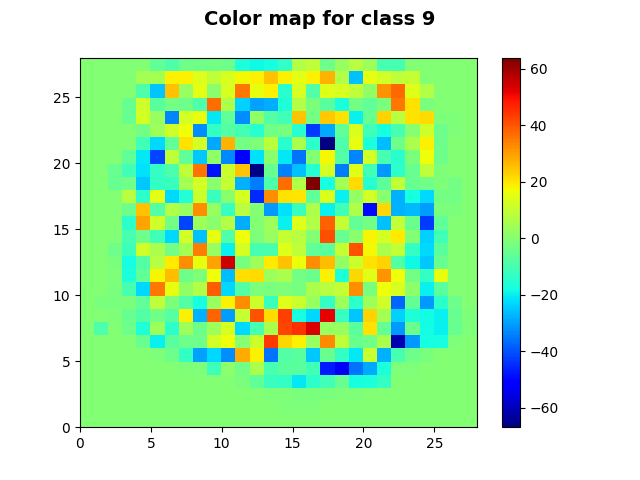
\includegraphics[scale=0.80]{part1.ec2/digit9.png}
\captionof{figure}{Color map for digit 9.}
\end{center}

In this visualizations, the high heat spots represent features that when present are very important to classify an example as the expected class and, in contrast, the lowest spots (scales of blue) indicate features that when present can help determine that an example is NOT of the given class; it doesn't tell anything about the right class, simply says that it may not be an example of a particular class.\\

\textbf{Extra Credit 3 - Differentiable weight update}: I decided to use the sigmoid function and apply the weight update from the slides:
\[ \vec{w} \leftarrow \vec{w} + \alpha (y - f(x))\sigma(\vec{w}\cdot \vec{x})(1 - \sigma(\vec{w}\cdot \vec{x}))\cdot \vec{x} \]

For calculating the $\sigma$ function I used the \textbf{expit} function from SciPy\footnote{\url{https://docs.scipy.org/doc/scipy-0.15.1/reference/generated/scipy.special.expit.html}}. \\

A few things to note from the results obtained using gradient descent:\\
\begin{enumerate}
\item The training curve obtained using sigmoid is smoother than the non-differentiable perceptron. This is congruent with intuition because the derivative tells you the "right" way in which to change the weights. Below you will find the training curve for the sigmoid perceptron.

\item The accuracy on the training data is not as high when using sigmoid, compared to the Part 1.1 perceptron.
\end{enumerate}

\begin{center}
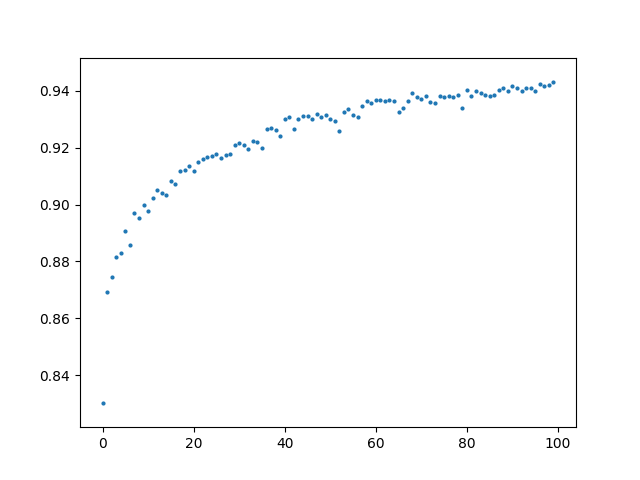
\includegraphics[scale=0.75]{part1.ec3/sigmoid-constant.png}
\captionof{figure}{Training curve for the perceptron using $\sigma$.}
\end{center}

Finally, the best accuracy achived using sigmoid was \textbf{82\%}, close to the best from Part 1.1. Additional experiments were performed trying to increase the accuracy without success. The attempts included increasing the number of epochs (this resulting in a higher accuracy for the training data but not considerable improvement in the test data), different $\alpha$ values and random weights initialization. The respective training curves can be found in the results folder but are not included here for brevity and because nothing more than a comparison was requested. \\

\textbf{Extra Credit 4 - Additional classifiers}: I decided to use scikit-learn\footnote{\url{http://scikit-learn.org/stable/}} to implement an SVM classifier. In particular, I used the SVC method that implements the "one-vs-one" approach instead of the "one-vs-other" implemented in my Perceptron classifier. For reference you can see \href{http://scikit-learn.org/stable/modules/generated/sklearn.svm.SVC.html#sklearn.svm.SVC}{this}. I tried different kernel functions to see how they impacted the accuracy of the model. There are four built-in kernel functions for SVC: rbf, sigmoid, linear and polynomial. \\

The following table summarizes the outcome of the different tries:
\begin{center}
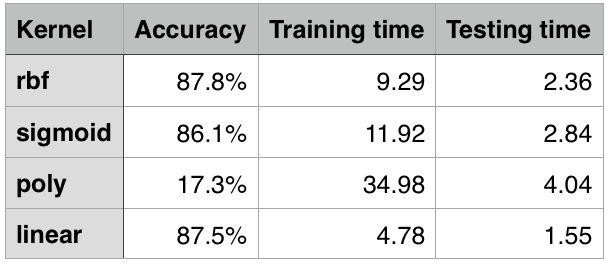
\includegraphics[scale=0.80]{part1.ec4/summary.png}
\captionof{figure}{Summary of the accuracies for SVC classification.}
\end{center}

Particularly interesting is the fact that a polynomial kernel gives a very bad accuracy while the other ones outperform my Perceptron classifier but not by a large margin.

\section*{Part 2}

\subsection*{Part 1.1}

\subsection*{Part 1.2}

\subsection*{Extra credits}

\end{document}
